
\documentclass[11pt,a4paper]{article}
\usepackage[utf8]{inputenc}
\usepackage[T1]{fontenc}
\usepackage[brazil]{babel}
\usepackage{amsmath, amssymb}
\usepackage{graphicx}
\usepackage{booktabs}
\usepackage{hyperref}
\usepackage{geometry}
\usepackage{xcolor}
\usepackage{listings}
\usepackage{caption}
\usepackage{csvsimple}
\usepackage[many]{tcolorbox}
\tcbuselibrary{listings, minted, breakable}
\usepackage{minted}

\setminted{
  breaklines,
  breakanywhere,
  fontsize=\footnotesize,
  linenos
}

\newtcblisting{BreakableCode}[2][]{%
  breakable,
  enhanced,
  minted language=python,
  minted options={breaklines, breakanywhere, linenos, fontsize=\footnotesize},
  colback=gray!3,
  colframe=gray!40,
  listing only,
  title={#2},
  #1
}

\geometry{margin=2.3cm}
\lstset{
  basicstyle=\ttfamily\footnotesize,
  breaklines=true,
  frame=single,
  numbers=left,
  numberstyle=\tiny,
  tabsize=2,
  showstringspaces=false
}
\renewcommand{\labelenumi}{\alph{enumi})} % Changes the label for the first level to (a), (b), etc.

\begin{document}
\begin{titlepage}
    \centering
    \vspace*{0.5cm}
    
\includegraphics[width=0.35\textwidth]{EP.jpg}\par\vspace{1cm}
    {\scshape\LARGE Escola Politécnica da Universidade de São Paulo \par}
    \vspace{1.2cm}
    {\scshape\Large PTC5725 -- Introdução aos Métodos Espectrais \par}
    \vspace{2.0cm}
    {\huge\bfseries Relatório: Tarefa complementar da aula 4\par}
    \vspace{2.0cm}
    {\Large Renan de Luca Avila\par}
    \vfill
    São Paulo, \today
\end{titlepage}

% Sumário
\tableofcontents
\clearpage

\section{Resumo}
Este documento contempla os 3 itens da tarefa complementar da aula 4.

\section{Enunciado}

\begin{enumerate}
    \item Resolver numericamente a seguinte ODE:
    \[
        x \in \Omega \equiv [1,3] \subset \mathbb{R} \text{ tal que } 
        \quad x\frac{du}{dx} + 2u = 4x^{2}, \quad \text{com } u(1)=2.
    \]
    \item Determine com a solução numérica o ponto 
    \[
        x \in [1,3] \quad \text{tal que} \quad u(x)=4,
    \]
    com pelo menos 10 dígitos de precisão.
    \item Compare o resultado com 
    \[
        x_k = \sqrt{\,2+\sqrt{3}\,}.
    \]
    Aproveite e mostre também que 
    \[
        x_k = 2\cos\!\left(\frac{\pi}{12}\right)
        = 2\sqrt{\frac{1+\cos(\pi/6)}{2}}.
    \]
\end{enumerate}

\section{Resolução do item \textit{a}}


\subsection{Solução analítica}

Primeiro, encontremos a solução analítica: consideremos o problema de valor inicial.
\[
x\,u'(x)+2u(x)=4x^{2}, \qquad u(1)=2, \qquad x\in[1,3].
\]

Como $x>0$ no domínio, multiplicamos a equação por $x$ e reconhecemos a derivada do produto no lado esquerdo da equação:
\begin{align*}
x^2 u'(x)+2x\,u(x) &= 4x^3,\\
\frac{d}{dx}\big(x^{2}u(x)\big) &= 4x^{3}.
\end{align*}

Integramos em $x$ dos dois lados:
\[
x^{2}u(x)=\int 4x^{3}\,dx = x^{4}+C
\quad\Longrightarrow\quad
u(x)=x^{2}+\frac{C}{x^{2}}.
\]

Aplicando a condição inicial $u(1)=2$:
\[
2 = 1 + C \;\;\Longrightarrow\;\; C=1.
\]

Portanto, a solução fechada é
\[
\boxed{\,u(x)=x^{2}+x^{-2}\,},\qquad x\in[1,3].
\]

\paragraph{Observação} Caso a ideia de multiplicar por $x$ dos dois lados pareça pouco intuitiva, o mesmo resultado surge pelo método padrão do fator integrante para EDO linear de 1ª ordem, usando $\mu(x)=\exp\!\big(\int \tfrac{2}{x}\,dx\big)=x^2$, o que leva novamente a $\frac{d}{dx}(x^2 u)=4x^3$.

\subsection{Solução numérica}

\paragraph{Planejamento}
Nesta etapa, nós vamos resolver numericamente a equação diferencial
\[
x\,u'(x)+2u(x)=4x^{2}, \qquad u(1)=2, \qquad x\in[1,3],
\]
utilizando o método de espectral de colocação de pontos de Chebyshev-Gauss-Lobatto.  
O domínio físico $x\in[1,3]$ é mapeado para o domínio computacional $\xi\in[-1,1]$ por meio da transformação linear
\[
x(\xi) = 2 + \xi, \qquad \frac{dx}{d\xi} = 1.
\]
Escolhemos $N+1$ pontos de colocação
\[
\xi_j = \cos\!\left(\frac{\pi j}{N}\right), \qquad j = 0,1,\dots,N,
\]
que são então mapeados para $x_j = 2 + \xi_j$.  
A matriz de derivada espectral $D$ é construída a partir da fórmula clássica de Chebyshev.  
A equação diferencial é discretizada nos nós internos conforme
\[
\mathrm{diag}(x)\,D\,\mathbf{u} + 2\,\mathbf{u} = 4\,\mathbf{x}^{\circ 2},
\]
e a condição de contorno $u(1)=2$ é imposta substituindo a primeira linha do sistema.  
Finalmente, nós vamos resolver o sistema linear para $\mathbf{u}$ e comparar com a solução analítica $u(x)=x^{2}+x^{-2}$, avaliando o erro pelo máximo da diferença absoluta.

\subsection{Construção do código}

Nesta subseção, nós conectamos o \emph{planejamento} da colocação de Chebyshev-Gauss–Lobatto à \emph{implementação} em Python (Listagem~\ref{lst:solucao_chebyshev}), explicando cada etapa e como ela aparece no código.

\paragraph{(1) Grade espectral e mapeamento do domínio.}
Planejamento: escolher pontos CGL em $\xi\in[-1,1]$ e mapear linearmente para $x\in[1,3]$ via $x(\xi)=2+\xi$.
No código:
\begin{verbatim}
xi = np.cos(np.pi * np.arange(N+1) / N)
x = 2 + xi
\end{verbatim}
Comentário: como $dx/d\xi=1$, a derivada em $x$ coincide com a derivada em $\xi$ na montagem da matriz.

\paragraph{(2) Matriz de derivada de Chebyshev $D$.}
Planejamento: construir $D$ clássica em CGL.
No código:
\begin{verbatim}
c = np.ones(N+1); c[0] = c[-1] = 2
D = np.zeros((N+1, N+1))
for i in range(N+1):
    for j in range(N+1):
        if i != j:
            D[i,j] = (c[i]/c[j]) * (-1)**(i+j) / (xi[i]-xi[j])
    D[i,i] = -np.sum(D[i,:])
\end{verbatim}
Isso implementa a fórmula padrão para $D$ em nós CGL, com correção dos termos diagonais para garantir que cada linha some a zero.

\paragraph{(3) Discretização da EDO nos nós internos.}
Planejamento: discretizar
\[
\mathrm{diag}(x)\,D\,\mathbf{u} + 2\,\mathbf{u} = 4\,\mathbf{x}^{\circ 2}.
\]
No código:
\begin{verbatim}
A = np.diag(x) @ D + 2*np.eye(N+1)
b = 4*x**2
\end{verbatim}
Aqui $A$ representa o operador discreto e $b$ o termo-força avaliado nos nós.

\paragraph{(4) Imposição da condição de contorno.}
Planejamento: impor $u(1)=2$ no nó de fronteira correspondente a $x=1$ (que é $\xi=-1$). No vetor \texttt{xi} usado, $\xi=-1$ é o \emph{último} nó, logo substituímos a última linha:
\begin{verbatim}
A[-1,:] = 0; A[-1,-1] = 1
b[-1] = 2
\end{verbatim}
Este passo implementa exatamente a estratégia planejada de substituir a equação de interior pela condição de contorno.

\paragraph{(5) Resolução do sistema e comparação com a solução analítica.}
Planejamento: resolver $A\mathbf{u}=\mathbf{b}$, computar erro e gerar figura.
No código:
\begin{verbatim}
u_num = np.linalg.solve(A, b)
u_ana = x**2 + 1/x**2
erro_max = np.max(np.abs(u_num - u_ana))
\end{verbatim}
Em seguida, a figura é produzida com as duas curvas (analítica e numérica) sobrepostas (Fig.~\ref{fig:solucao_chebyshev}).

\subsection{Implementação em Python.}

Código em \ref{lst:solucao_chebyshev}.

\begin{listing}[tbp]
    \inputminted[
        frame=lines,
        framesep=2mm,
        baselinestretch=1.1,
        bgcolor=gray!5,
        fontsize=\footnotesize,
        linenos
    ]{python}{code/solucao_chebyshev.py}
    \caption{Implementação em Python do método de colocação de Chebyshev-Gauss-Lobatto.}
    \label{lst:solucao_chebyshev}
\end{listing}

\begin{figure}
    \centering
    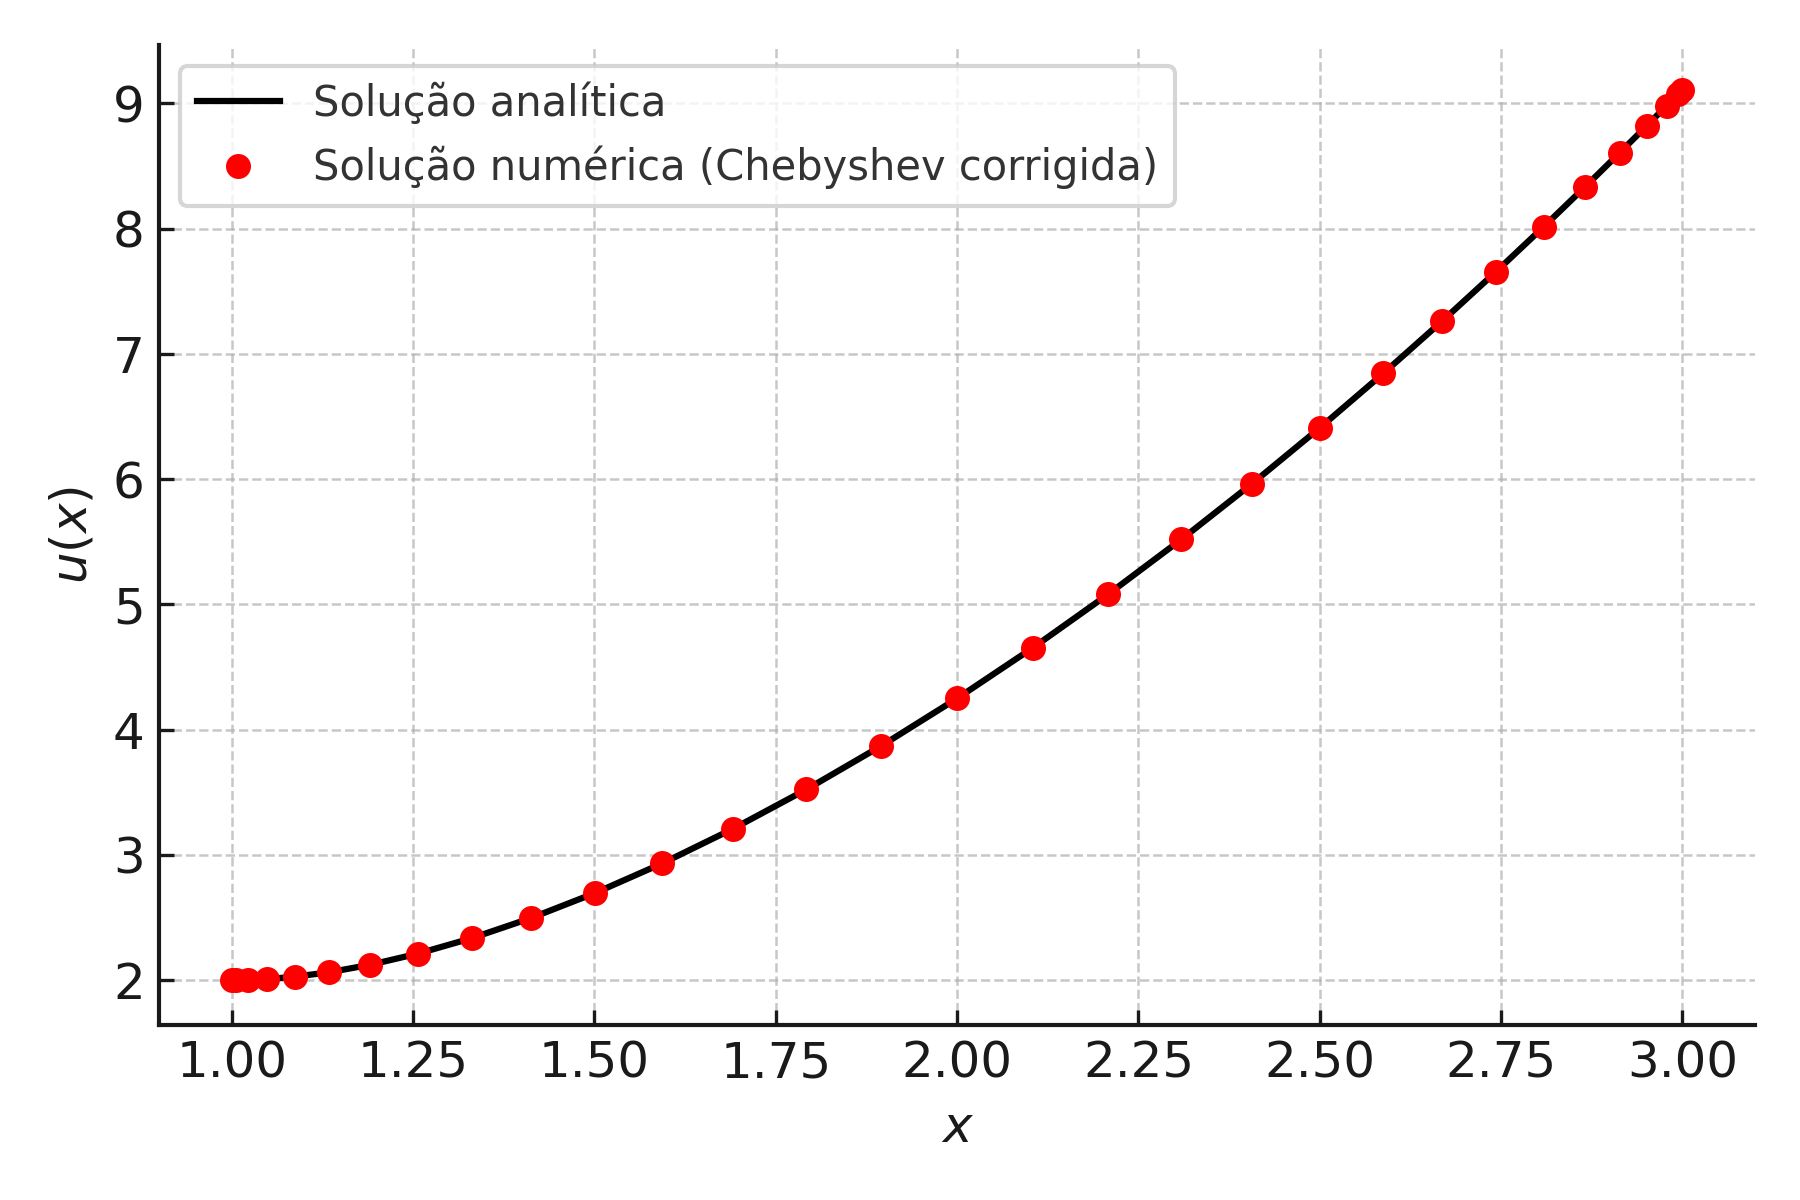
\includegraphics[width=0.65\textwidth]{figures/fig_solucao_chebyshev.png}
    \caption{Comparação entre a solução analítica $u(x)=x^{2}+x^{-2}$ e a solução numérica obtida pelo método de colocação de Chebyshev-Gauss-Lobatto.}
    \label{fig:solucao_chebyshev}
\end{figure}

\subsection{Conclusão.}

Na \autoref{fig:solucao_chebyshev} apresentamos a comparação entre a solução analítica e a solução numérica obtida pelo método de colocação.  
O método apresentou excelente concordância: o erro máximo entre ambas as soluções foi da ordem de $10^{-11}$, evidenciando a alta precisão espectral do método.

Observamos que a solução numérica obtida pelo método de colocação de Chebyshev-Gauss-Lobatto reproduz a solução analítica praticamente sem erro perceptível, o que confirma a eficiência e a convergência espectral do método para equações diferenciais lineares suaves.  
A discretização com apenas $N=30$ pontos já fornece precisão de aproximadamente $10^{-11}$ no domínio $[1,3]$, o que valida a metodologia empregada.

\subsection{Extensão voluntária: estudo de convergência do erro com $N$}

\paragraph{Planejamento.}
Nós vamos medir o erro máximo 
$\|u_{\text{num}}-u_{\text{ana}}\|_{\infty}
=\max_j |u_{\text{num}}(x_j)-u_{\text{ana}}(x_j)|$
nos nós de Chebyshev-Gauss-Lobatto mapeados para $[1,3]$, variando o grau $N$ do polinômio (número de pontos $N{+}1$) em uma sequência aproximadamente exponencial (valores pequenos até moderados). A expectativa teórica para problemas suaves é de \emph{convergência espectral} (erro decaindo de forma quase-exponencial em $N$).

\paragraph{Resultados.}
A \autoref{fig:erro_vs_N_cheb} mostra o erro máximo em escala logarítmica. Observa-se queda rápida desde $N\approx 6$ até atingir o “plateau” de erro de máquina (dupla precisão) por volta de $N\in[24,32]$.

\begin{figure}[H]
    \centering
    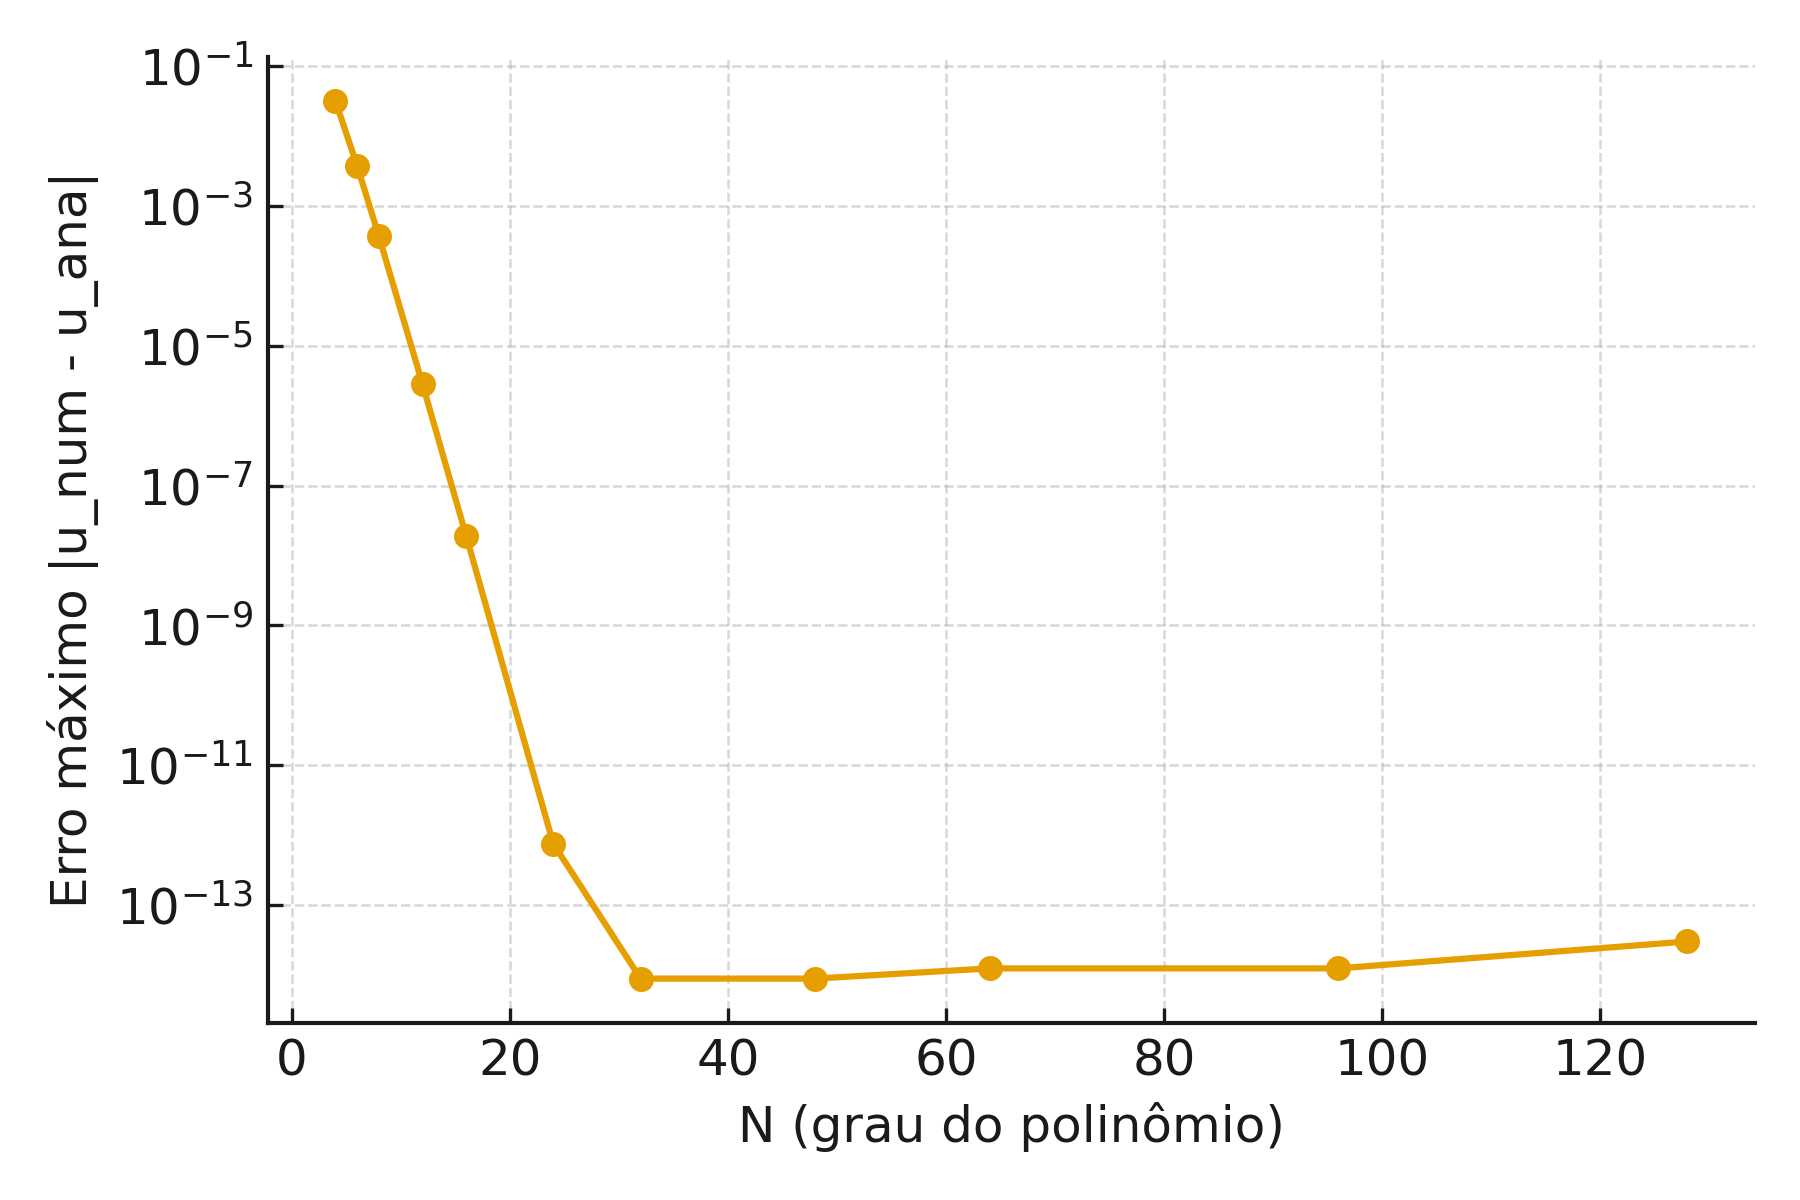
\includegraphics[width=0.65\textwidth]{figures/erro_vs_N_chebyshev.png}
    \caption{Erro máximo $\|u_{\text{num}}-u_{\text{ana}}\|_{\infty}$ em função de $N$ para a colocação de Chebyshev-Gauss-Lobatto. Nota-se convergência espectral até a saturação pelo erro de arredondamento.}
    \label{fig:erro_vs_N_cheb}
\end{figure}

\paragraph{Conclusão.}
Com poucos pontos ($N\approx 24$ a $32$), já atingimos erros próximos de $10^{-13}$ a $10^{-14}$, o que confirma a eficiência do método para esta EDO suave. Mas em valores de $N$ maiores, o erro deixa de diminuir, o que é curioso e motiva a seguinte seção de estudo.

\subsubsection{Saturação do erro}

A \autoref{fig:erro_teorico_componentes_final} ilustra, de forma conceitual, o comportamento típico do erro em métodos espectrais quando aumentamos o número de pontos de colocação $N$.  
Observamos duas componentes principais do erro:

\begin{itemize}
    \item \textbf{Erro de truncamento} ($E_{\mathrm{trunc}}$): decai exponencialmente com $N$, representando a precisão teórica do método espectral. Nos primeiros valores de $N$, essa é a componente dominante do erro.
    \item \textbf{Erro de arredondamento} ($E_{\mathrm{round}}$): é inerente à aritmética de ponto flutuante. Ele permanece praticamente constante enquanto o erro de truncamento é grande, mas passa a dominar quando o erro de truncamento se aproxima do limite de precisão de máquina.
\end{itemize}

A curva do erro total $E(N)$ (linha preta) evidencia três regimes distintos:

\begin{enumerate}
    \item \textbf{Regime I – Convergência inicial:} o erro é controlado pelo truncamento e decai exponencialmente;
    \item \textbf{Regime II – Saturação:} o erro atinge o piso numérico, não diminuindo mais mesmo com o aumento de $N$;
    \item \textbf{Regime III – Crescimento numérico:} pequenas instabilidades e o mau condicionamento do operador espectral fazem o erro total crescer levemente.
\end{enumerate}

Portanto, mesmo que o erro de arredondamento esteja presente desde o início, ele é insignificante em $N$ pequenos e só se torna relevante quando o método alcança o limite da precisão de máquina.  
A figura demonstra claramente esse fenômeno: o erro total exibe uma forma côncava, decaindo rapidamente até cerca de $N \approx 80$ e, em seguida, estabilizando devido à saturação numérica.

\begin{figure}[H]
    \centering
    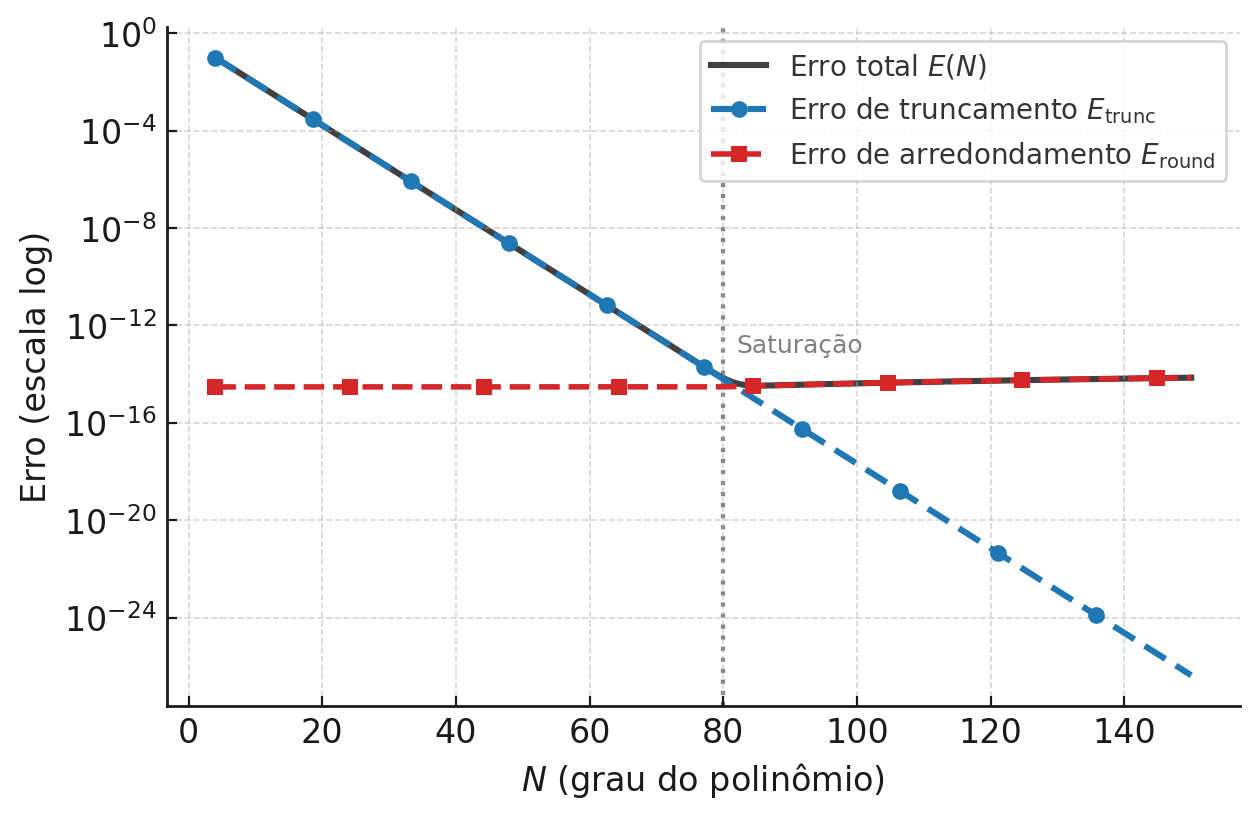
\includegraphics[width=0.68\textwidth]{figures/fig_erro_teorico.png}
    \caption{Comportamento conceitual (ilustrativo) do erro de truncamento ($E_{\mathrm{trunc}}$), do erro de arredondamento ($E_{\mathrm{round}}$) e do erro total ($E(N)$). O ponto de saturação numérica ocorre quando $E_{\mathrm{trunc}} \approx E_{\mathrm{round}}$, em torno de $N \approx 80$.} Note que o erro de arredondamento após a saturação cresce.
    \label{fig:erro_teorico_componentes_final}
\end{figure}

Além do fenômeno de saturação do erro, o erro de truncamento também pode se comportar mau a depender do método utilizado em situações específicas, o que nos faz questionar as limitações do método de colocação de pontos de Chebyshev e motiva a próxima seção de estudos.

\subsubsection{Limitações específicas do método de colocação de Chebyshev-Gauss–Lobatto}

Embora o método de colocação de Chebyshev apresente excelente precisão e convergência espectral para funções suaves, ele possui limitações intrínsecas que devem ser consideradas:

\paragraph{(i) Aglomeração de nós nos extremos.}
Os pontos de Chebyshev-Gauss–Lobatto se distribuem de forma não uniforme, com forte concentração nas vizinhanças das fronteiras.  
Essa característica é vantajosa para a imposição de condições de contorno, mas pode levar a uma amostragem excessiva nas extremidades e escassez de pontos na região central, afetando a resolução de fenômenos localizados no interior do domínio.

\paragraph{(ii) Condicionamento das matrizes diferenciais.}
As matrizes de derivada de Chebyshev tornam-se rapidamente mal-condicionadas à medida que $N$ aumenta.  
Em particular, o número de condicionamento cresce aproximadamente como
\[
\kappa(D^{(1)}) = \mathcal{O}(N^2), 
\qquad 
\kappa(D^{(2)}) = \mathcal{O}(N^4),
\]
o que implica amplificação de erros de arredondamento na solução numérica do sistema linear associado.  
Na prática, isso limita o número de pontos utilizável antes que o erro de máquina comece a dominar (regime de saturação).

\begin{small}
\noindent \textbf{Nota sobre o número de condicionamento.} \;
O símbolo $\kappa(A)$ denota o \emph{número de condicionamento} de uma matriz $A$, definido por
\[
\kappa(A) = \|A\|_2 \, \|A^{-1}\|_2,
\]
onde $\|\cdot\|_2$ representa a norma induzida pela norma euclidiana (equivalente ao maior valor singular).
Esse número mede a sensibilidade da solução do sistema linear $A x = b$ a pequenas perturbações nos dados:
\[
\frac{\|\delta x\|}{\|x\|} \lesssim \kappa(A)\,
\frac{\|\delta b\|}{\|b\|}.
\]
Valores pequenos de $\kappa(A)$ indicam que o sistema é bem condicionado, 
enquanto valores grandes implicam amplificação de erros de arredondamento e perda de precisão numérica. 
No contexto das matrizes diferenciais de Chebyshev, o crescimento de $\kappa(D^{(m)})$ com $N$ explica a degradação da estabilidade numérica e a saturação do erro para grandes ordens de colocação.
\end{small}

\paragraph{(iii) Saturação da precisão para grandes $N$.}
Mesmo para funções suaves, o aumento de $N$ não garante melhoria indefinida de precisão.  
Após certo ponto, o erro de truncamento torna-se menor que o erro de arredondamento, e o método atinge um \emph{piso numérico}, observado experimentalmente na Figura~\ref{fig:erro_teorico_componentes_final}.  
Esse fenômeno é típico de discretizações baseadas em derivadas espectrais de Chebyshev.

\paragraph{(iv) Sensibilidade a erros de mapeamento.}
O método depende fortemente da transformação $x(\xi)$ entre o domínio físico e o domínio padrão $[-1,1]$.  
Pequenos erros de escala ou mapeamentos mal escolhidos podem alterar a distribuição efetiva dos nós e afetar tanto a estabilidade quanto a precisão da solução.

\paragraph{(v) Custo computacional e preenchimento denso.}
As matrizes diferenciais de Chebyshev são densas, o que implica custo computacional $\mathcal{O}(N^2)$ para operações básicas e $\mathcal{O}(N^3)$ para a resolução direta de sistemas lineares.  
Diferentemente de discretizações locais (como diferenças finitas), o método de colocação não se beneficia de esparsidade estrutural.

\medskip
\noindent
\textbf{Em resumo}, o método de colocação de Chebyshev é extremamente eficiente e preciso para problemas suaves e de baixa ordem, mas apresenta limitações práticas associadas ao condicionamento, à concentração de nós e à saturação de precisão.  
Esses fatores devem orientar a escolha de $N$ e a estratégia de implementação numérica.

\section{Resolução do item \textit{b}}

\paragraph{Planejamento} Encontrar a raiz via interpolante baricêntrico e Newton--Raphson.

\paragraph{Código.}
O código a seguir implementa:
(i) a solução por colocação CGL,
(ii) a construção do interpolante baricêntrico $p_N(x)$ e de sua derivada $p_N'(x)$,
(iii) o método de Newton--Raphson aplicado a $f(x)=p_N(x)-4$.

\inputminted[
  breaklines,
  breakanywhere,
  linenos,
  fontsize=\footnotesize,
  frame=lines,
  framesep=2mm,
  baselinestretch=1.05
]{python}{code/barycentric_newton_root.py}

\paragraph{Visual.}
A solução analítica $u(x)=x^2+x^{-2}$ e o interpolante baricêntrico $p_N(x)$, com as linhas de nível $u=4$ e as posições das raízes analítica e numérica, estão na Fig.~\ref{fig:root_barycentric_newton}:
\begin{figure}[tbp]
  \centering
  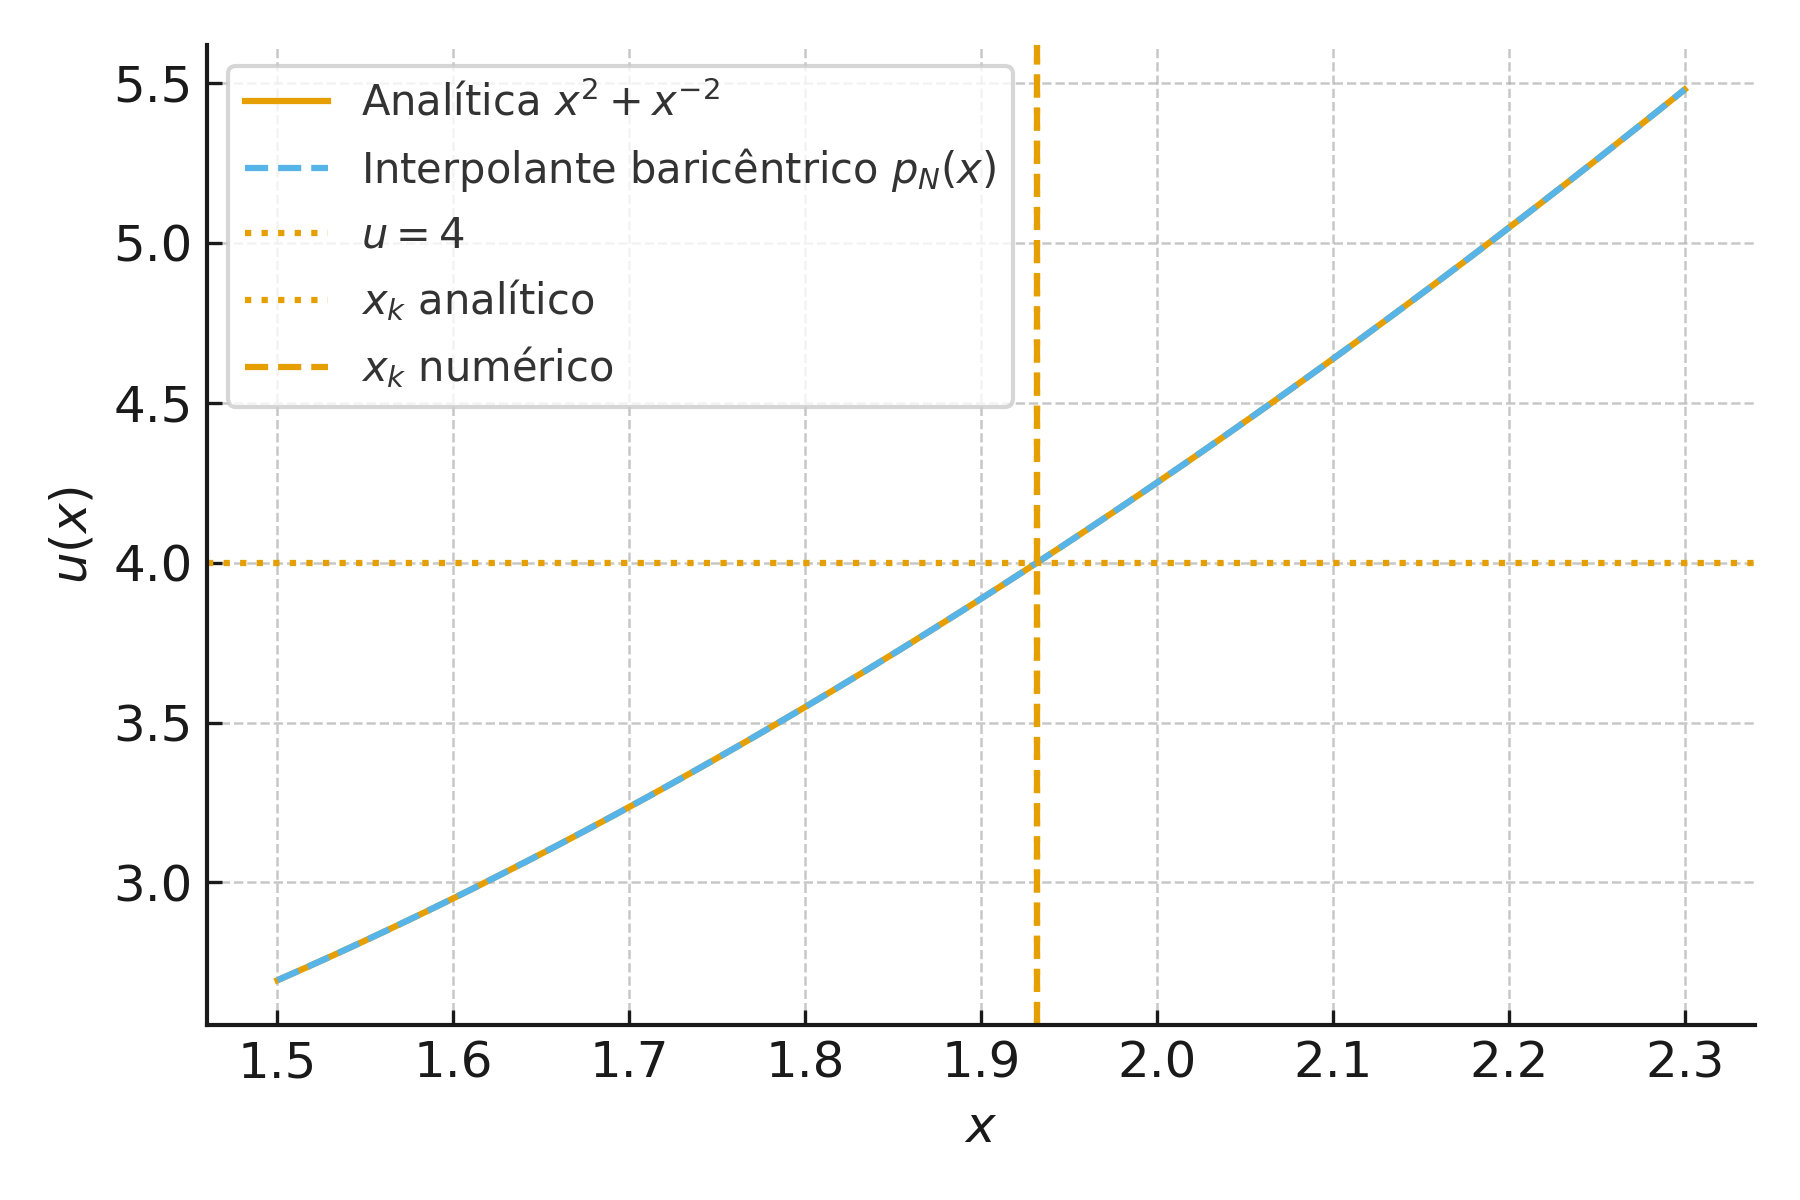
\includegraphics[width=0.70\textwidth]{figures/fig_root_barycentric_newton.png}
  \caption{Interpolante baricêntrico $p_N(x)$ (CGL) e solução analítica $u(x)=x^2+x^{-2}$. A interseção com $u=4$ fornece a raiz $x_k$.}
  \label{fig:root_barycentric_newton}
\end{figure}

\paragraph{Histórico do método de Newton e critério de parada.}
O histórico de iterações é apresentado na Tabela \ref{tab:newton_history}. 

\begin{listing}[tbp]
\caption{Histórico de Newton na busca da raiz de $p_N(x)-4=0$.}
\label{tab:newton_history}
\begin{center}
\csvautotabular{tables/newton_barycentric_history.csv}
\end{center}
\end{listing}

No experimento reportado, o método convergiu em \textbf{5 iterações} com o critério de parada
\[
\lvert p_N(x_k)-4\rvert < 10^{-13} \quad \text{(máximo: 50 iterações).}
\]
A raiz numérica encontrada coincide com a solução analítica $x_k=\sqrt{2+\sqrt{3}}$ até o piso de máquina.

A raiz analítica é 
\[
x_k=\sqrt{2+\sqrt{3}}= \mathbf{1.9318516525781366}\,.
\]
Usando o interpolante baricêntrico com Newton--Raphson (CGL, $N=30$), obtivemos a estimativa numérica
\[
x_N=\mathbf{1.9318516525781364}\,,
\]
o que resulta em erro absoluto
\[
|x_N-x_k|=\mathbf{2.220446049250313\times 10^{-16}},
\]
compatível com o piso de precisão em dupla.

\section{Resolução do item \textit{c}}

Do item (b), o valor fechado é
\[
x_k=\sqrt{\,2+\sqrt{3}\,}.
\]

\paragraph{Equivalência.}
Mostremos que
\[
\sqrt{\,2+\sqrt{3}\,} \;=\; \frac{\sqrt{6}+\sqrt{2}}{2}.
\]
De fato,
\[
\left(\frac{\sqrt{6}+\sqrt{2}}{2}\right)^{\!2}
=\frac{6+2+2\sqrt{12}}{4}
=\frac{8+4\sqrt{3}}{4}
=2+\sqrt{3}.
\]
Como ambos os lados são positivos, segue a igualdade desejada:
\[
\boxed{\,x_k=\sqrt{\,2+\sqrt{3}\,}=\dfrac{\sqrt{6}+\sqrt{2}}{2}\,}.
\]
\paragraph{Observação: possível relação com trigonometria?}
Usando a identidade de ângulo-diferença,
\[
\cos(15^\circ)=\cos(45^\circ-30^\circ)
=\cos 45^\circ\,\cos 30^\circ+\sin 45^\circ\,\sin 30^\circ
=\frac{\sqrt{2}}{2}\cdot\frac{\sqrt{3}}{2}+\frac{\sqrt{2}}{2}\cdot\frac{1}{2}
=\frac{\sqrt{6}+\sqrt{2}}{4}.
\]
Logo,
\[
2\cos\!\left(\frac{\pi}{12}\right)=2\cos(15^\circ)
=\frac{\sqrt{6}+\sqrt{2}}{2}
=\sqrt{\,2+\sqrt{3}\,}.
\]
Portanto,
\[
\boxed{\,x_k=\sqrt{\,2+\sqrt{3}\,}=2\cos\!\left(\frac{\pi}{12}\right)\,}.
\]


\paragraph{Conclusão.}
As expressões acima mostram que as diferentes formas radicais para $x_k$ são exatamente equivalentes e coerentes com o valor fechado obtido no item (b). E talvez exista alguma relação do problema original com alguma peculiaridade trigonométrica.

\section{Ambiente Python: instalação e execução dos scripts}

Nesta seção, nós vamos configurar um ambiente Python isolado, instalar as bibliotecas necessárias e executar os scripts do projeto. As instruções abaixo cobrem Windows, macOS e Linux.

\subsection{ Instalar o Python (3.10+ recomendado)}
\begin{itemize}
  \item \textbf{Windows}: baixe o instalador em \texttt{https://www.python.org/downloads/} e marque a opção \emph{“Add Python to PATH”}.
  \item \textbf{macOS}: use o instalador oficial ou o Homebrew: \verb|brew install python|.
  \item \textbf{Linux}: use o gerenciador de pacotes (\emph{e.g.}, Ubuntu: \verb|sudo apt-get install python3 python3-venv python3-pip|).
\end{itemize}
Para verificar: \verb|python --version| (ou \verb|python3 --version|).

\subsection{ Criar e ativar um ambiente virtual}
No diretório raiz do seu projeto (aquele que contém \texttt{code/}, \texttt{figures/} e \texttt{tables/}), nós vamos criar um \emph{virtualenv}:
\begin{verbatim}
# Windows (PowerShell)
python -m venv .venv
.\.venv\Scripts\Activate.ps1

# macOS / Linux (bash/zsh)
python3 -m venv .venv
source .venv/bin/activate
\end{verbatim}
Se a ativação funcionar, o prompt exibirá algo como \texttt{(.venv)} à esquerda.

\subsection{ Instalar as dependências}
Nós vamos usar apenas bibliotecas padrão para os gráficos e manipulação de dados. Crie um arquivo \texttt{requirements.txt} (ou copie o bloco abaixo) e instale:
\begin{verbatim}
# requirements.txt
numpy>=1.24
matplotlib>=3.7
pandas>=2.0
\end{verbatim}
Instalação:
\begin{verbatim}
pip install --upgrade pip
pip install -r requirements.txt
\end{verbatim}

\subsection{Executar os scripts do projeto}
Após a instalação, nós vamos executar os scripts (eles geram automaticamente figuras em \texttt{figures/} e tabelas em \texttt{tables/}):
\begin{verbatim}
# Solução numérica por colocação e figura comparativa
python code/solucao_chebyshev_corrigida.py

# Estudo de convergência do erro vs N (gera CSV e figura)
python code/erro_vs_N_chebyshev.py

# Raiz do item (b) via interpolante baricêntrico + Newton (gera CSV e figura)
python code/barycentric_newton_root.py
\end{verbatim}
Caso seu sistema use \verb|python3| como comando padrão, substitua \verb|python| por \verb|python3|.

\subsection{ Onde encontrar as saídas}
\begin{itemize}
  \item \textbf{Figuras}: \texttt{figures/fig\_solucao\_chebyshev\_corrigida.png}, \texttt{figures/erro\_vs\_N\_chebyshev.png}, \texttt{figures/fig\_root\_barycentric\_newton.png}.
  \item \textbf{Tabelas (CSV)}: \texttt{tables/erro\_convergencia\_cheb.csv}, \texttt{tables/newton\_barycentric\_history.csv}.
  \item \textbf{Resumo (texto)}: \texttt{result\_barycentric\_newton.txt} (com raiz analítica, raiz numérica e erro).
\end{itemize}

\section{Reconhecimento de Uso de LLM}

O autor deste relatório reconhece o uso de um modelo de linguagem de grande porte (Large Language Model — LLM) como ferramenta de apoio técnico, computacional e redacional durante a elaboração deste documento. 

O LLM (ChatGPT, da OpenAI) foi utilizado para:
\begin{itemize}
  \item gerar descrições teóricas e explicações matemáticas a partir dos conceitos estudados na disciplina;
  \item estruturar o relatório em seções, tabelas e figuras com coerência técnica e formal;
  \item auxiliar na formatação \LaTeX, integração de códigos e visualizações numéricas;
  \item revisar consistência e clareza textual.
\end{itemize}

Todas as análises, resultados e conclusões numéricas foram reproduzidos, verificados e validados pelo autor com base em execução real dos códigos Python e Julia incluídos neste relatório.


\end{document}
